% {\color{red} Need paraphrase to avoid self-plagiarism\color{blue}

This section presents a construction of a $(k,s)$-RdB sequence $\bfc_{k,s}$. Furthermore, given a substring of length $k$ of the sequence $\bfc_{k,s}$, a fast decoding algorithm to determine the location of the given substring is provided. The complexity of the decoding algorithm is sub-linear with respect to the length of $\bfc_{k,s}$. There are some classical de Bruijn sequences with sub-linear decoding algorithm \cite{mitchell1996method,tuliani2001bruijn,kociumaka2016efficient}. This work uses the minimal de Bruijn sequence, constructed in \cite{kociumaka2016efficient,fredricksen1978necklaces}, and some special properties of Lyndon words to construct a $(k,s)$-RdB.
% }

\begin{definition}[\textbf{Lyndon words}]
    A sequence $w$ is a Lyndon word if and only if it's strictly smaller than all of its rotation.
\end{definition}
For more intelligible, several Lyndon words and non-Lyndon words are provided in example~\ref{exp:Lyndon}.
\begin{example}[Lyndon words]\label{exp:Lyndon}
    The word $00101$ is a Lyndon word since it is smaller than all of its rotations: $01010$, $10100$, $01001$, $10010$. The word $01100$ is not a Lyndon word, since one of its rotations, $00011$, is smaller than it. The word $011011$ is also not a Lyndon word, as its cyclic rotation by $3$ letters is equal to it. 
\end{example}

\subsection{Encoder for a\texorpdfstring{$(k,s)$}{(k,s)}-RdB sequence} \label{subsect:encoder}
In 1978, Fredricksen and Maiorana~\cite{fredricksen1978necklaces} proposed the \gls{fkm} algorithm to efficiently construct the lexicographically minimal de Bruijn sequence, which is later called the granddaddy sequence by Knuth~\cite{knuth2013art}. The algorithm was based on their finding of the connection between the de Bruijn sequence and Lyndon words.

\begin{lemma}[\cite{fredricksen1978necklaces}]\label{lem:FKM}
    The lexicographically minimal de Bruijn sequence of order $k$ ($k$-MdB) is the concatenation of all Lyndon words whose length is a divisor of $k$ in the lexicographical order.
\end{lemma}

For example, the $6$-MdB sequence is decomposed into Lyndon words as follows:
\begin{example}[Decomposition of $6$-MdB sequence]
    Recall that $6$-MdB sequence is already given in example~\ref{exp:granddaddy}, which is:
    \[0000001000011000101000111001001011001101001111010101110110111111\]

    As stated in lemma~\ref{lem:FKM}, it can be decomposed in lexicographically order into Lyndon words listed follows:
    \begin{align*}
        &0\\
        &000001\\
        &000011\\
        &000101\\
        &000111\\
        &001\\
        &001011\\
        &001101\\
        &001111\\
        &01\\
        &010111\\
        &011\\
        &011111\\
        &1
    \end{align*}
\end{example}


This thesis observes that it is able to append a prefix to a suffix of $k$-MdB to obtain a $(k,s)$-RdB sequence, i.e., in the cycle representing $k$-MdB, there are arcs representing $(k,s)$-RdB sequences. To illustrate this idea, figure~\ref{fig:substring_of_circle} gives an example for $k=6$ and $s=2$, where the blue arc and the red arc indicate the prefix and the suffix respectively. Any substring of the concatenation of the prefix and suffix is a $(6,2)$-RdB sequence.

\begin{figure}[htbp]
    \centering
    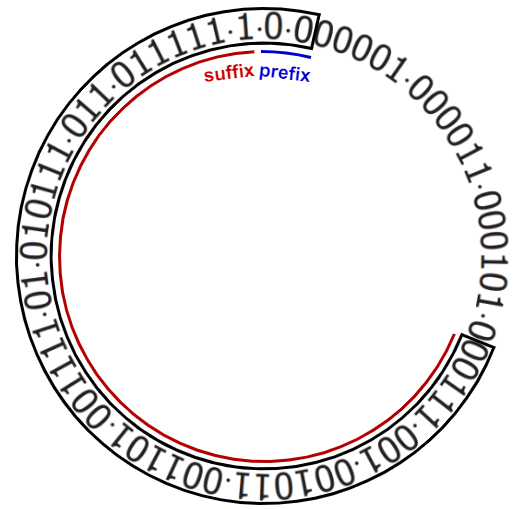
\includegraphics[scale=0.5]{fig/construction/subtring of cyclic.png}
    \caption{Example for $k=6,\ s=2$. In the circle of $6$-MdB, an arbitrary substring of the concatenation of suffix and prefix in the picture is a $(6,2)$-RdB sequence.}
    \label{fig:substring_of_circle}
\end{figure}

% \begin{figure}
%     \centering
%     \input{fig/construction/construction}
%     \caption{Caption}
%     \label{fig:my_label}
% \end{figure}

More precisely, the construction is described as follows:
\begin{construction}\label{constr:encoder}
    Let $\bfx=(x_{1},\ldots,x_{n})$ be the $k$-MdB constructed from Lemma~\ref{lem:FKM} and $u_{k,s}= 0^{s+1}1^{k-s-1}$ be a Lyndon word of length $k$ satisfying the first $s+1$ letters are all $0$'s and the last $k-s-1$ letters are all $1$'s. By the intrinsic property of de Bruijn sequences, there exists only one index $i$ such that $\bfu_{k,s}=\bfx[i,i+k-1]=(x_{i},\ldots,x_{i+k-1})$. Denote the word $\bfc_{k,s} = (x_{i+1},\ldots,x_{n},0,0,\ldots,0)$, obtained by adding $s$ letters $0$ to the end of the suffix of $\bfx$, from index $i+1$ to the end. Theorem \ref{theo:validity} below claims that $\bfc_{k,s}$ is a $(k,s)$-RdB sequence. 
\end{construction}

This thesis later proves that $\bfc_{k,s}$ is even the longest $(k,s)$-RdB sequence. 

Denote \L$_{n}$ to be the set of all Lyndon words of length $n$, and $\text{\L}^{(n)}=\cup_{d\card n}\text{\L}_{d}$ to be the set of all Lyndon words whose lengths are divisors of n. The formal encoder to construct a $(k,s)$-RdB sequence is given in algorithm~\ref{alg:encoder}.

\begin{algorithm}
\DontPrintSemicolon
    \SetKwInOut{KwIn}{Input}
    \SetKwInOut{KwOut}{Output}
    \KwIn{$k$, and descending ordered set \L$^{(n)}$. }
    \KwOut{ $(k,s)$-RLL dBs}
    \BlankLine
        % Find the set of Lyndon words  $S=\left\{\lambda_{i}:\ \lambda_{i}\in\mathsf{L}^{(k)}\right\}$
    
    $\mathbf{w}\gets$emptystring\;
    \For{$\lambda \in$\L$^{(n)}$}{
        $\mathbf{w}.prepend(\lambda)$\;
        \If{$\lambda== 0^{s+1}1^{k-s-1}$}{
            \tcc{remove the first letter of $w$, which is 0, and add $s$ letters $0$ to the end}
            $\mathbf{w} = \mathbf{w}[2,\ell]0^{s}$\;
            \textbf{break}\;
        }
    }
    \KwRet{$\mathbf{w}$}
    \caption{Encode (k,s)-RLL dBs}
    \label{alg:encoder}
\end{algorithm}

The set $\text{\L}^{(n)}$ in lexicographically order can be generated in constant amortized time by applying \gls{fkm} algorithm (analyzed in~\cite{ruskey1992generating}), or by another algorithm developed by Duval in~\cite{duval1988generation}. In algorithm~\ref{alg:encoder}, the most consuming time step is to produce the set $\text{\L}^{(n)}$, and hence, its complexity is the complexity of the algorithm used to bring out $\text{\L}^{(n)}$.
% {\color{red} Runtime of Encoder, critical runtime is at FKM ...}

Here presents an example for $k=6$ and $s=2$. 
\begin{example}[Construction of $(6,2)$-RdB sequence]
    The suffix: $$00111\ 001011\ 001101\ 001111\ 01\ 010111\ 011\ 011111\ 1$$ is taken from the granddaddy of order $6$ given above. Adding $2$ letter $0$ to the end of it obtains:
    \[
        00111\ 00\ 001011\ 001101\ 001111\ 01\ 010111\ 011\ 011111\ 1\ 00
    \]
    which is indeed a $(6,2)$-RdB sequence.
\end{example}
Now, theorem \ref{theo:validity} proves that the Construction~\ref{constr:encoder} always return a $(k,s)$-RdB sequence.

\begin{theorem}\label{theo:validity}
    The sequence $\bfc_{k,s}$ obtained from Construction~\ref{constr:encoder} is a $(k,s)$-RdB sequence.
\end{theorem}
\begin{proof}
    First, it's necessary to show that each substring of length $k$ appears at most once in $\bfc_{k,s}$. Note that the granddaddy sequence $\bfx$ obtained from Lemma~\ref{lem:FKM} is a cyclic de Bruijn sequence, and $\bfc_{k,s}$ is actually a substring of $\bfx$. Hence, $\bfc_{k,s}$ just contains each substring of size $k$ at most once.
    
    Now, claiming that $\bfc_{k,s}$ doesn't contain any patterns $0^{s+1}$ will complete the theorem. This can be proved by considering the property of Lyndon words. It's obvious to see that $\bfu_{k,s}=0^{s+1}1^{k-s-1}$ is the largest Lyndon word containing $s+1$ consecutive symbols $0$. Hence, every Lyndon word decomposed from $\bfc_{k,s}$ doesn't take $0^{s+1}$ as a substring. Moreover, the last symbol of all Lyndon words but $0$ is $1$. Therefore, $0^{s+1}$ will not appear in the combination of Lyndon words larger than $\bfu_{k,s}$. Adding $0^{s}1^{k-s-1}$ to the beginning and $s$ letters $0$ to the end of this combination resulting in $\bfc_{k,s}$ won't change this property. So, it's able to conclude that $\bfc_{k,s}$ is indeed a $(k,s)$-RdB sequence.
\end{proof}

\subsection{Decoder for a \texorpdfstring{$(k,s)$}{(k,s)}-RdB sequence}
In~\cite{zhang2021timing}, the Hybrid de Bruijn sequence of order $k$ after being received needs to be decoded for correcting errors. More particularly, it's necessary to indicate the exact location of an arbitrary sequence of length $k$ in the Hybrid de Bruijn sequence. To do that, they proposed to use a look-up table, which is an exponential complex method.

Similarly, it's essential for this work to decode $\bfc_{k,s}$. In 2016, Kociumaka, Radoszewski, and Rytter presented the first sub-linear decoding algorithm $\cD_{KRR}$ for the minimal de Bruijn sequences. And since $\bfc_{k,s}$ is a substring of a minimal de Bruijn sequence, it's able to modify $\cD_{KRR}$ to decode $\bfc_{k,s}$ in sub-linear time. 

Let $i=\cD_{KRR}(\bfu_{k,s})$ be the position of the word $\bfu_{k,s}$ in the granddaddy sequence of order $k$ $\bfx$. Recall that, from Construction~\ref{constr:encoder}, we have $\bfc_{k,s}=(x_{i+1},\ldots,x_{n},0^{s})$. Thus, for each length $k$ word $v$ lying in $\bfc_{k,s}$, its location in $\bfc_{k,s}$ is to location of $v$ in $x$ minus $j$, unless they are of the form $1^{j}0^{k-j}$ for all $1\leq j\leq s$ which appear at the end of $\bfc_{k,s}$. The formal description of our decoding algorithm is shown in algorithm \ref{alg:decode}.

\begin{algorithm}
\DontPrintSemicolon
    \SetKwInOut{KwIn}{Input}
    \SetKwInOut{KwOut}{Output}
    \KwIn{A word $\bfv=(v_1,\ldots,v_k)$ of length $k$}
    \KwOut{a is the location of $\bfv$ in $\bf\bfc_{k,s}$}
    \BlankLine
    
    $i \gets \cD_{KRR}(\bfu_{k,s})$; \\
     \tcc{ $\cD_{KRR}$ is the decoder of the minimal de Bruijn sequence in \cite{kociumaka2016efficient}}
     \If {$\bfv = 1^{j}0^{k-j}$,}{\KwRet{$n-i+1-(k-j)$};}
     \Else{\KwRet{$\cD_{KRR}(\bfv)-i$};}
    \caption{Decode (k,s)-RdB $\bf\bfc_{k,s}$}
    \label{alg:decode}
\end{algorithm}

\subsection{The optimality of our construction}
This section gives proof for the claim stated in section \ref{sec:graph_representation}, that is, the encoder produces sequence $\bfc_{k,s}$ whose length equals to to upper bound $\mathcal{U}(k,s)$, and thus, $\bfc_{k,s}$ is the longest the $(k,s)$-RdB sequence. In order to do so, $\bfc_{k,s}$'s length, denoted by $\ell(\bfc_{k,s})$, is needed calculating first. It's then essential to show that $\ell(\bfc_{k,s})$ is equal to $\mathcal{U}(k,s)$ by some algebraic transformations.

Given a word $\bfu$, denote $\langle \bfu\rangle$ to be its minimal rotation. For instance, the minimal rotation of 010110 is 001011, or, the minimal rotation of 010101 is itself. For every word $\bfv$, we define:
\begin{align*}
    S(\bfv) = \left\{\bfu: \bfu\in\Sigma^{\card{ \bfv}},\langle \bfu\rangle\leq \bfv\right\}
\end{align*}
to be the set of all sequence of length $\card{ \bfv}$ satisfying their minimal rotation doesn't exceed $\bfv$. The following example~\ref{exp:S_v} lists all element of $S(\bfv)$ with $\bfv=01101$.
\begin{example}[Example of $S(\bfv)$]\label{exp:S_v}
    Given $\bfv= 01101$, all sequence of length $\card{\bfv}=5$ whose minimal rotations are at most $\bfv$ is:
    \begin{align*}
        S(01101) = \bigl\{ &00000,\\
        &00001,00010,00100,01000,10000, \\
        &00011,00110,01100,11000,10001, \\
        &00111,01110,11100,11001,10011 \bigl\}
    \end{align*}
\end{example}
If $\bfv$ is a Lyndon word, Lemma 29 in \cite{kociumaka2016efficient} tells that the cardinality of $S(\bfv)$, $\card{ S(\bfv)}$, equals to the length of the prefix of the granddaddy sequence $\bfx$, from the beginning to the sub-string $\bfv$. Recall that $\bfu_{k,s}$ is also a Lyndon word, one has:
\begin{align}
    \card{ S(\bfu_{k,s})} &= 2^{k}- (\ell(\bfc_{k,s}) - (k-1) -s ) \nonumber\\
    \Leftrightarrow  \ell(\bfc_{k,s}) &= 2^{k}+(k-1)+s-\card{ S(\bfu_{k,s})} \label{eq:cks&sks}
\end{align}

This brings the idea determining $\ell(\bfc_{k,s})$ by computing the size of the set $S(\bfu_{k,s})$. 
\begin{lemma}\label{lem:card_S_uks}
    Let $A_{t} = 2^{t-2}$ for all $t>1$, $A_{1}=1$, and $M=\max{(k-s,s+3)}$. Then:
    \begin{align}
        \card{ S(\bfu_{k,s})}= 1 + \sum_{t=M}^{k}(k-t+1)\card{C(t-2,s)} + \sum_{t=1}^{k-s-1}A_{t} \label{eq:card_S_uks}
    \end{align}
\end{lemma}
\begin{proof}
    Let $i,j$ be two non-negative integers such that $i+j<k$, denote:
    $$U_{i,j}= \left\{0^{i}1x1_{t}0^{j}\in S(\bfu_{k,s}): i+j+t=k\right\}$$
    to be the set of all words in $S(\bfu_{k,s})$ satisfying its prefix of length $i+1$ is $0^{i}1$ and its suffix of length $j+1$ is $10^{j}$.
    
    Since $S(\bfu_{k,s})$ is the disjoint union of $0^k$ and all sets $U_{i,j}$ for $i,j \geq 0$ and $i+j<k$, we obtain:
    \begin{equation}\label{eq:s=1+2u}
        \card{S(\bfu_{k,s})}= 1 +\sum_{\substack{i,j\geq 0 ; i+j \leq s}} \card{U_{i,j}}+\sum_{\substack{i,j\geq 0 ; s < i+j<k}} \card{U_{i,j}}.
    \end{equation}
    
    If we fix $1\leq t \leq k$, there are $k-t+1$ pairs $(i,j)$ such that $t=k-i-j$. If $i+j \leq s$ then the sub-string $1x1_{t}$ must contain $s+1$ consecutive 0's (consequently, $k-i-1-(i+2)+1\geq s+1\Rightarrow t=k-i-j\geq s+3$), and therefore, $\card{U_{i,j}}=\card{C(t-2,s)}.$ 
    Hence,
    \begin{equation}\label{eq:c1}
        \cC_1= \sum_{\substack{i,j\geq 0 ;\\ i+j \leq s}} \card{U_{i,j}} = \sum_{t=M}^{k}(k-t+1)\card{C(t-2,s)}. 
    \end{equation}
    where $M=\max(s+3,k-s)$.
    
    If $k>i+j > s$ then the sub-string $(x_{i+2},\ldots,x_{k-j-1})$ can be any word of length $t-2$ and thus $\card{U_{i,j}}=A_t=2^{t-2}$. Hence:
    \begin{equation}\label{eq:c2}
        \cC_2=\sum_{\substack{i,j\geq 0 ;\\ s< i+j<k}} \card{U_{i,j}}= \sum_{t=1}^{k-s-1}(k-t+1)A_{t}.
    \end{equation}
    From Equations (\ref{eq:s=1+2u}), (\ref{eq:c1}), (\ref{eq:c2}), we get the result in Lemma \ref{lem:card_S_uks}.
\end{proof}

Combining the results from Lemma~\ref{lem:card_S_uks} and equation~\ref{eq:cks&sks} gives: 
\begin{align*}
    \ell(\bfc_{k,s}) = 2^{k}+k+s-2-\cC_{1}-\cC_{2}
\end{align*}
where $\cC_{1}$ and $\cC_{2}$ are defined in Equation~\ref{eq:c1} and \ref{eq:c2}. It's now ready to prove the following lemma, which states that the proposed construction is optimal.
\begin{lemma}\label{lemma:2_length_equal}
    The length the sequence $\bfc_{k,s}$ returned from Construction~\ref{constr:encoder} is optimal, that is:
    \begin{align}
        \ell(\bfc_{k,s}) = \mathcal{U}(k,s) \label{eq:equals_lowerbound}
    \end{align}
\end{lemma}
\begin{proof}
    Equation~\ref{eq:equals_lowerbound} is equivalent to:
    \begin{align}
        2^{k}+k+s-2-\cC_{1}-\cC_{2} &= \card{ W(k,s)} - \left(\sum_{i=0}^{C}\card{ W(k-i-d-3,s)} - s\right) +(k-1) \nonumber\\
        \Leftrightarrow 2^{k} - (1+\cC_{1}+\cC_{2}) &= \card{W(k,s)} - \left( \sum_{i=0}^{C}\card{ W(k-i-d-3,s)} \right) \label{eq:2length_equal_v2}
    \end{align}
    First, the value of $C$ and $M$ is necessarily explicated by considering the relation between $k$ and $s$. In short, there are $3$ following cases:
    \[
    \left\{\begin{matrix}
        M=k-s,\ C = s-1\ \text{if\ } s+3\leq k-s\\
        M=s+3,\ C = s-1\ \text{if\ } k=2s+2,s<k-1\\
        M=s+2,\ C = k-s-2\ \text{if\ } k\leq 2s+1
    \end{matrix}\right.
    \]
    \textbf{Case 1}: $M=k-s,\ C = s-1\ \text{when\ } s+3\leq k-s$. The equation needing to be proved \ref{eq:2length_equal_v2} becomes:
    \begin{align*}
        &\card{W(k,s)} - \left(\sum_{i=0}^{s-1}(s-i)\card{W(k-s-i-3,s)}\right) \\
        =\ &2^{k}-\left(1+\sum_{t=k-s}^{k}(k-t+1)\card{C(t-2,s)}+\sum_{t=1}^{k-(s+1)}(k-t+1)A_{t}\right)
    \end{align*}
    In the right hand side, recall that $\card{C(t-2,s)} = 2^{t-2}-\card{ W(t-2,s)}$, so:
    \begin{align*}
        \mathrm{\gls{rhs}} &= 2^{k}-\left(1+\sum_{t=k-s}^{k}(k-t+1)\card {C(t-2,s)}+\sum_{t=1}^{k-(s+1)}(k-t+1)A_{t}\right)\\
        &=2^{k} - \left(1+\sum_{t=1}^{k}(k-t+1)A_{t}-\sum_{t=k-s}^{k}(k-t+1)\card{W(t-2,s)}\right)\\
        &=2^{k} - \left(2^{k}-\sum_{t=k-s}^{k}(k-t+1)\card{W(t-2,s)}\right)\\
        &(\text{the term }1+\sum_{t=1}^{k}(k-t+1)A_{t} \text{ can be easily shown to be equal to } 2^{k})\\
        &= \sum_{t=k-s}^{k}(k-t+1)\card{W(t-2,s)}
    \end{align*}
    Thus: \[\mathrm{\gls{lhs}}=\mathrm{\gls{rhs}}\]
    \[\Leftrightarrow \card{W(k,s)} - \left(\sum_{i=0}^{s-1}(s-i)\card{ W(k-s-i-3,s)} \right) = \sum_{t=k-s}^{k}(k-t+1)\card{ W(t-2,s)}\]
    \[\Leftrightarrow \card{W(k,s)} = \sum_{t=2}^{s+2}(t-1)\card{W(k-t,s)} + \sum_{t=s+3}^{2s+2}(2s+3-t)\card{ W(k-t,s)}\ (*)\]
    Recall that:
    \begin{align*}
        \card{W(k,s)} &= \sum_{i=1}^{s+1}\card{ W(k-i,s)}\ \forall k>s\\
        &=\card{ W(k-1,s)}+\card{ W(k-2,s)} + \cdots + \card{ W(k-s-1,s)}\ \forall k>s
    \end{align*}
    Therefore, when $k\geq2s+3$, the following system of equations is obtained:
    \[\left\{\begin{matrix}
        \card{ W(k-1,s)} = &\card{ W(k-2,s)} + \card{ W(k-3,s)}+\cdots + \card{ W(k-s-2,s)} \\
        \card{ W(k-2,s)} = &\card{ W(k-3,s)} + \card{ W(k-4,s)}+\cdots + \card{ W(k-s-3,s)} \\
        \cdots \\
        \card{ W(k-s-1,s)} = &\card{ W(k-s-2,s)} + \card{ W(k-s-3,s)}+\cdots + \card{ W(k-2s-2,s)}
    \end{matrix}\right.\]
    Adding side by side the above equations results in the equation $(*)$, which is needed to be verified.
    
    \textbf{Case 2}: $M=s+3,\ C=s-1$ when $k=2s+2,s<k-1$. 
    The \gls{lhs} is the same as in the first case, meanwhile, the \gls{rhs} is :
    \begin{align*}
        \mathrm{\gls{rhs}} = &2^{k}-\left(1+\sum_{t=s+3}^{2s+2}(k-t+1)\card{ C(t-2,s)}+\sum_{t=1}^{k-(s+1)}(k-t+1)A_{t}\right) \\
        =&2^{k}-\left(1+\sum_{t=1}^{2s+2}A_{t}-\sum_{t=s+3}^{2s+2}(k-t+1)\card{ W(t-2,s)}-(s+1)2^{s}\right)\\
        =&\sum_{t=s+2}^{2s+2}(k-t+1)\card{ W(t-2,s)}\\
        =&\sum_{t=k-s}^{k}(k-t+1)\card{ W(t-2,s)}
    \end{align*}
    what's left to be proved is similar to the first case.
    
    \textbf{Case 3}: $M=s+3,\ C=k-s-2$ when $s+2\leq k\leq 2s+1$.
    Again, the \gls{rhs} is $\mathrm{\gls{rhs}} = \sum_{t=k-s}^{k}(k-t+1)\card{ W(t-2,s)}$, and the LHS is:
    \[\card{ W(k,s)} - \left(\sum_{i=0}^{k-s-2}(s-i)\card{ W(k-s-i-3,s)} \right)\]
    Therefore:
    \[\mathrm{\gls{lhs}} = \mathrm{\gls{rhs}}\]
    \[\Leftrightarrow \card{ W(k,s)} = \sum_{t=2}^{s+2}(t-1)\card{ W(k-t,s)} + \sum_{t=s+3}^{k+1}(2s+3-t)\card{ W(k-t,s)} (**)\]
    The situation is quite similar to the first case, and recall that : $\card{ W(n,s) } = 2^{s}\ \forall 0\leq n\leq s$, $\card{ W(-1,s)} = 1$. Thus:
    
    \[\left\{\begin{matrix}
        \card{ W(k-1,s)} &= \card{ W(k-2,s)} + \card{ W(k-3,s)}+\ldots + \card{ W(k-s-2,s)} \\
        \card{ W(k-2,s)} &= \card{ W(k-3,s)} + \card{ W(k-4,s)}+\ldots + \card{ W(k-s-3,s)} \\
        \cdots \\
        \card{ W(k-t,s)} &= \card{ W(k-t-1,s)} + \card{ W(k-t-2,s)}+\ldots + \card{ W(k-t-s-1,s)},\\ \text{with } k-t=s+1  \\
        \card{ W(k-t-1,s)} &= \card{ W(k-t-2,s)} + \card{ W(k-t-3,s)}+\ldots + \card{ W(0,s)} +\card{ W(-1,s)}\\
        \cdots\\
        \card{ W(k-s-1,s)} &= \card{ W(k-s-2,s)} + \card{ W(k-s-3,s)} +\ldots+ \card{ W(-1,s)} \\
    \end{matrix}\right.\]

    Once again, adding side by side the above equations gives $(**)$.
    
    In conclusion, in all $3$ cases, the correctness of equation \ref{eq:2length_equal_v2} is verified, hence, Lemma~\ref{lemma:2_length_equal} is proved.
\end{proof}
